% Created 2021-02-21 Sun 12:24
% Intended LaTeX compiler: pdflatex
\documentclass[a4paper,11pt,twoside]{article}
\usepackage[utf8]{inputenc}
\usepackage[T1]{fontenc}
\usepackage{graphicx}
\usepackage{grffile}
\usepackage{longtable}
\usepackage{wrapfig}
\usepackage{rotating}
\usepackage[normalem]{ulem}
\usepackage{amsmath}
\usepackage{textcomp}
\usepackage{amssymb}
\usepackage{capt-of}
\usepackage{hyperref}
\usepackage{minted}
\IfFileExists{./resources/style.sty}{\usepackage{./resources/style}}{}
\IfFileExists{./resources/referencing.sty}{\usepackage{./resources/referencing}}{}
\addbibresource{../resources/references.bib}
\usepackage[mode=buildnew]{standalone}
\usepackage{tikz}
\usetikzlibrary{decorations.fractals}
\usetikzlibrary{lindenmayersystems}
\author{Ryan Greenup}
\date{\today}
\title{Implementing of RankNet}
\hypersetup{
 pdfauthor={Ryan Greenup},
 pdftitle={Implementing of RankNet},
 pdfkeywords={},
 pdfsubject={},
 pdfcreator={Emacs 28.0.50 (Org mode 9.4.4)}, 
 pdflang={English}}
\begin{document}

\maketitle
\tableofcontents

\# \#+TODO: TODO IN-PROGRESS WAITING DONE
 \newpage 

\section{Introduction}
\label{sec:orgc564536}
Ranknet is an approach to \emph{Machine-Learned Ranking (often refered to
as "\emph{/Learning to Rank}}" \cite{liuLearningRankInformation2009}) that
began development at Microsoft from 2004 onwards
\cite{christopherburgesRankNetRankingRetrospective2015}, although
previous work in this area had already been undertaken as early as
the 90s (see generally
\cite{fuhrProbabilisticModelsInformation1992,fuhrOptimumPolynomialRetrieval1989,fuhrProbabilisticModelsInformation1992,geyInferringProbabilityRelevance1994,wongLinearStructureInformation1988})
these earlier models didn't perform well compared to more modern
machine learning techniques
\cite[\S 15.5]{manningIntroductionInformationRetrieval2008}.

Information retrieval is an area that demands effective ranking of
queries, although straight-forward tools such as \texttt{grep}, relational
databases (e.g. sqlite, MariaDB, PostgreSql) or NoSQL (e.g. CouchDB,
MongoDB) can be used to retrieve documents with matching characters
and words, these methods do not perform well in real word tasks
across large collections of documents because they do not provide
any logic to rank results (see generally
\cite{viksinghComparisonOpenSource2009}).


\section{Motivation}
\label{sec:org6285c98}

Search Engines implement more sophisticated techniques to rank
results, one such example being TF-IDF weighting
\cite{martyschochBleveSearchDocumentation} , well established
search engines such as \emph{Apache Lucene}
\cite{apachesoftwarefoundationLearningRankApache2017} and \emph{Xapian}
\cite{jamesaylettGSoCProjectIdeasLearningtoRankStabilisationXapian2019},
however, 
are implementing Machine-Learned Ranking in order to improve results.

This paper hopes to serve as a general introduction to the implementation
of the Ranknet technique to facilitate developers of search engines in
more modern languages (i.e. \texttt{Go} and \texttt{Rust}) in implementing
it. This is important because these more modern languages are more
accessible \cite{huntThesisSubmittedPartial}
and memory safe \cite{perkelWhyScientistsAre2020} than C/C++
respectfully, without significantly impeding performance; this will
encourage contributors from more diverse backgrounds and hence
improve the quality of profession-specific tooling.


For a non-comprehensive list of actively maintained search engines,
see \S \ref{sec:orgc3c7fd7} of the appendix.

\section{Implementation}
\label{sec:orgaaf6f78}



Neural Networks 

Ranking/ is the process of applying machine learning algorithms to
ranking problems, it .

This implementation will first apply the approach to a simple data
set so as to clearly demonstrate that the approach works, following
that the model will be extended to support wider and more complex
data types before finally being implemented on a corpus of documents.

\subsection{Neural Networks}
\label{sec:org8033a53}

The Ranknet method is typically implemented using a Neural Networks
\footnote{An early goal of this research was to evaluate the performance
of different machine learning algorithms to implement the Ranknet
method, as well as contrasting this with simple classification
approaches, this research however is still ongoing,  see \S
\ref{sec:orgbab0c14}},
although other machine learning techniques can also be used
\cite[p. 1]{christopherburgesRankNetRankingRetrospective2015},
Neural Networks are essentially a collection of different
regression models and classifiers that are fed into one another to create a
non-linear classifier, a loss function is used to measure the
performance of the model with respect to the parameters
(e.g. RMSE \footnote{\textbf{RMSE} \emph{Root Mean Square Error}} or BCE \footnote{\textbf{BCE} \emph{Binary Cross Entropy}}) and the parameters are adjusted so
as to reduce this error by using the \emph{Gradient Descent Technique}
(although there are other optimisation algorithms such as RMSProp
and AdaGrad \cite{mukkamalaVariantsRMSPropAdagrad2017} that can be
shown to perform better, see
\cite{bushaevUnderstandingRMSpropFaster2018}). The specifics of
Neural Networks are beyond the scope of this paper (see
\cite{hmkcodeBackpropagationStepStep} or more generally \cite{pictonNeuralNetworks1994}).

\subsubsection{The Ranknet Method}
\label{sec:org4c8a3dd}

The Ranknet method is concerned with a value \(p_{ij}\) that
measures the probability that an observation \(i\) is ranked higher
than an observation \(j\).

A Neural Network (\(n\)) is trained to return a value
\(s_k\) from a feature vector \(\mathbf{X}_k\):

 \[n(\mathbf{X}_i) = s_i \quad \exists k\]
So as to minimise the error of:




\begin{align} 
 p_{ij} &= \mathrm{sig}\left(\sigma, (s_i-s_j) \right) \quad \exists \sigma \in \mathbb{R} \\
 &\text{where:} \nonumber \\
 &\quad  \mathrm{sig}\left(\sigma, x\right) = \frac{1}{1+e^{\sigma \cdot x}} 
\end{align} 



\paragraph{Version Control}
\label{sec:org6f630f1}
The implementation in this paper corresponds to the \texttt{walkthrough} branch
of the \texttt{git} repository used in production of this work, id values
(e.g. \texttt{:08db5b0:}) will be appended to titles to denote specific
changes made in that section. See \S \ref{sec:org466ef15} for
more specific guidance.

\paragraph{Code listings}
\label{sec:org5d2fb5b}
The code listings provided will use a standard set of import
statements (see \S \ref{sec:orgd262b36} ) and so they will be
omitted from the listings, for more comprehensive guidance on
implementing this code refer to the \href{https://crmds.github.io/CRMDS-HDR-Training-2020/}{documentation page}\footnote{\href{https://crmds.github.io/CRMDS-HDR-Training-2020/}{crmds.github.io/CRMDS-HDR-Training-2020/}} that
accompanies the \texttt{git} repo.

\subsection{Creating Data\hfill{}\textsc{cf9ab26}}
\label{sec:org7e4bbf4}
The first step is to create a simple data set and design a neural
network that can classify that data set, the data set generated
should have two classes of data (this could be interpreted as
relevant and irrelevant documents given the features or principle
components of a data set), this can be implemented using sci kit
learn as shown below and visualized\footnote{See \S \ref{sec:org66415ad} for the specific method definition used to
export the data to a \texttt{csv.}} in figure \ref{fig:orga2c4a64}.\footnote{Visualisations for this Report were implemented using
\texttt{org-babel} \cite{dominikOrgModeReference2018} inside \emph{Emacs}
\cite{stallmanGNUEmacsManual2002} to call \textbf{\emph{R}}
\cite{rcoreteamLanguageEnvironmentStatistical2021} with \emph{GGPlot2}
\cite{wickhamGgplot2ElegantGraphics2016a} (and \emph{Tidyverse}
\cite{wickhamWelcomeTidyverse2019} generally), the source code for this
is avaliable in the report manuscript available in the \texttt{git} repository
available at \href{https://github.com/RyanGreenup/ranknet/blob/main/Report/Report.org}{github.com/RyanGreenup/ranknet/blob/main/Report/Report.org}}


In order to fit a Neural Network the \emph{PyTorch} package can be used
\cite{NEURIPS2019_9015}, this will allow the gradients of the neural
network to be calculated numerically without needing to solve for
the partial derivatives, hence the data will need to be in the
form of tensors.

\begin{minted}[]{python}
def make_data(create_plot=False, n=1000, dtype=torch.float, dev="cpu", export=""):
    X, y = datasets.make_blobs(n, 2, 2, random_state=7)
    # X, y = datasets.make_moons(n_samples=n, noise=0.1, random_state=0) # Moons Data for later

    # Save the data somewhere if necessary
    if export != "":
	export_data(X, y, export)

    # Reshape the data to be consistent
    y = np.reshape(y, (len(y), 1))  # Make y vertical n x 1 matrix.

    # -- Split data into Training and Test Sets --------------------
    data = train_test_split(X, y, test_size=0.4)

    if(create_plot):
	# Create the Scatter Plot
	plt.scatter(X[:, 0], X[:, 1], c=y)
	plt.title("Sample Data")
	plt.show()

    # Make sure we're working with tensors not mere numpy arrays
    torch_data = [None]*len(data)
    for i in range(len(data)):
	torch_data[i] = torch.tensor(data[i], dtype=dtype, requires_grad=False)

    return torch_data

# Set Torch Parameters
dtype = torch.float
dev = test_cuda()

# Generate the Data
X_train, X_test, y_train, y_test = make_data(
    n=int(300/0.4), create_plot=True, dtype=dtype, dev=dev, export = "/tmp/simData.csv")
\end{minted}


\begin{figure}[htbp]
\centering
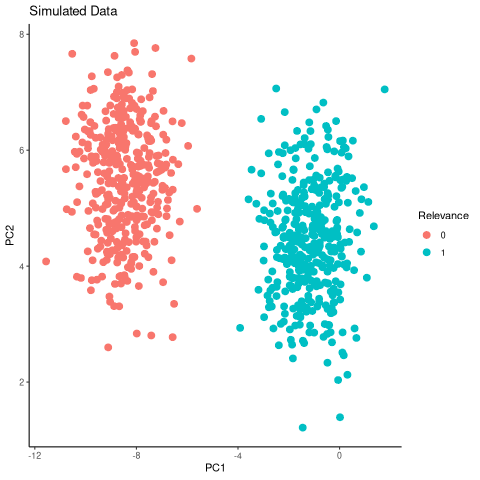
\includegraphics[width=0.4\textwidth]{SimulatedData.png}
\caption{\label{fig:orga2c4a64}Generated data, output classes denote document relevance and the axis features or principle components}
\end{figure}

\subsection{Creating a Neural Network\hfill{}\textsc{7291112}}
\label{sec:org4fa7e5f}
A Neural Network model can be designed as a class, here a 2-layer
model using Sigmoid functions has been described, this design was
chosen for it's relative simplicity:

\begin{minted}[]{python}
class three_layer_classification_network(nn.Module):
    def __init__(self, input_size, hidden_size, output_size, dtype=torch.float, dev="cpu"):
	super(three_layer_ranknet_network, self).__init__()
	self.wi = torch.randn(input_size, hidden_size,
			      dtype=dtype,
			      requires_grad=True,
			      device=dev)
	self.wo = torch.randn(hidden_size, output_size,
			      dtype=dtype,
			      requires_grad=True,
			      device=dev)

	self.bi = torch.randn(hidden_size,
			      dtype=dtype,
			      requires_grad=True,
			      device=dev)
	self.bo = torch.randn(output_size,
			      dtype=dtype,
			      requires_grad=True,
			      device=dev)

	self.σ = torch.randn(1, dtype=dtype, requires_grad=True, device=dev)

	self.losses = []       # List of running loss values
	self.trainedQ = False  # Has the model been trained yet?

    def forward(self, x):
	x = torch.matmul(x, self.wi).add(self.bi)
	x = torch.sigmoid(x)
	x = torch.matmul(x, self.wo).add(self.bo)
	x = torch.sigmoid(x)
	return x

    def loss_fn(self, x, y):
	y_pred = self.forward(x)
	return torch.mean(torch.pow((y-y_pred), 2))

    def misclassification_rate(self, x, y):
	y_pred = (self.forward(x) > 0.5)
	return np.average(y != y_pred)
\end{minted}

A model can then be instantiated, a \texttt{2-3-1}
model has, arbitrarily, been implemented in this case:\footnote{note that the model has not yet been trained, the weights are
random and the model output is not related to the data at all.}

\begin{minted}[]{python}
# Set Seeds
torch.manual_seed(1)
np.random.seed(1)

# Set Torch Parameters
dtype = torch.float
dev = test_cuda()

# Make the Data
X_train, X_test, y_train, y_test = make_data(
    n=100, create_plot=True, dtype=dtype, dev=dev)

# Create a model object
model = three_layer_classification_network(
    input_size=X_train.shape[1], hidden_size=2, output_size=1, dtype=dtype, dev=dev)

# Send some data through the model
print("\nThe Network input is:\n---\n")
print(X_train[7,:], "\n")
print("The Network Output is:\n---\n")
print(model.forward(X_train[7,:]).item(), "\n")

\end{minted}

\begin{verbatim}
The Network input is:
---

tensor([-1.5129,  2.9332]) 

The Network Output is:
---

0.22973690927028656 
\end{verbatim}

\subsection{Train the Model with Gradient Descent\hfill{}\textsc{7d46636}}
\label{sec:orged1d681}
Now that the model has been fit, a method to train the model can be
implmented \footnote{This class definition is incomplete and serves only to show the
method definition corresponding to the original class shown in \S
\ref{sec:org4fa7e5f}}:
\begin{minted}[]{python}
class three_layer_classification_network(nn.Module):
    # __init__ method goes here, see above
    # ...
    # ...

    def train(self, x, target, η=30, iterations=2e4):
	bar = Bar('Processing', max=iterations) # progress bar
	for t in range(int(iterations)):

	    # Calculate y, forward pass
	    y_pred = self.forward(x)

	    # Measure the loss
	    loss = self.loss_fn(x, target)

	    # print(loss.item())
	    self.losses.append(loss.item())

	    # Calculate the Gradients with Autograd
	    loss.backward()

	    with torch.no_grad():
		# Update the Weights with Gradient Descent 
		self.wi -= η * self.wi.grad; self.wi.grad = None
		self.bi -= η * self.bi.grad; self.bi.grad = None
		self.wo -= η * self.wo.grad; self.wo.grad = None
		self.bo -= η * self.bo.grad; self.bo.grad = None
		self.σ  -= η * self.σ.grad;  self.σ.grad = None
	    bar.next()
	bar.finish()
		# ; Zero out the gradients, they've been used

    # Rest of the Class Definition Below ...VVV...
\end{minted}

With this definition the model can hence be trained in order to
produce meaningful classifications, as shown below, this model classifies the
points perfectly, even on the testing data, the training error 
over time is shown in figure \ref{fig:org5f8c32b}.

\begin{minted}[]{python}
# Make the Data
X_train, X_test, y_train, y_test = make_data(
    n=100, create_plot=True, dtype=dtype, dev=dev)

# Create a model object
model = three_layer_classification_network(
    input_size=X_train.shape[1], hidden_size=2, output_size=1, dtype=dtype, dev=dev)

# Train the Model
model.train(X_train, y_train, η=1e-2, iterations=10000)

# Plot the losses
plt.plot(model.losses)
plt.title("Losses at each training iteration")
plt.show()

print("The testing misclassification rate is:\n")
print(model.misclassification_rate(X_test, y_test))
\end{minted}


\begin{figure}[htbp]
\centering
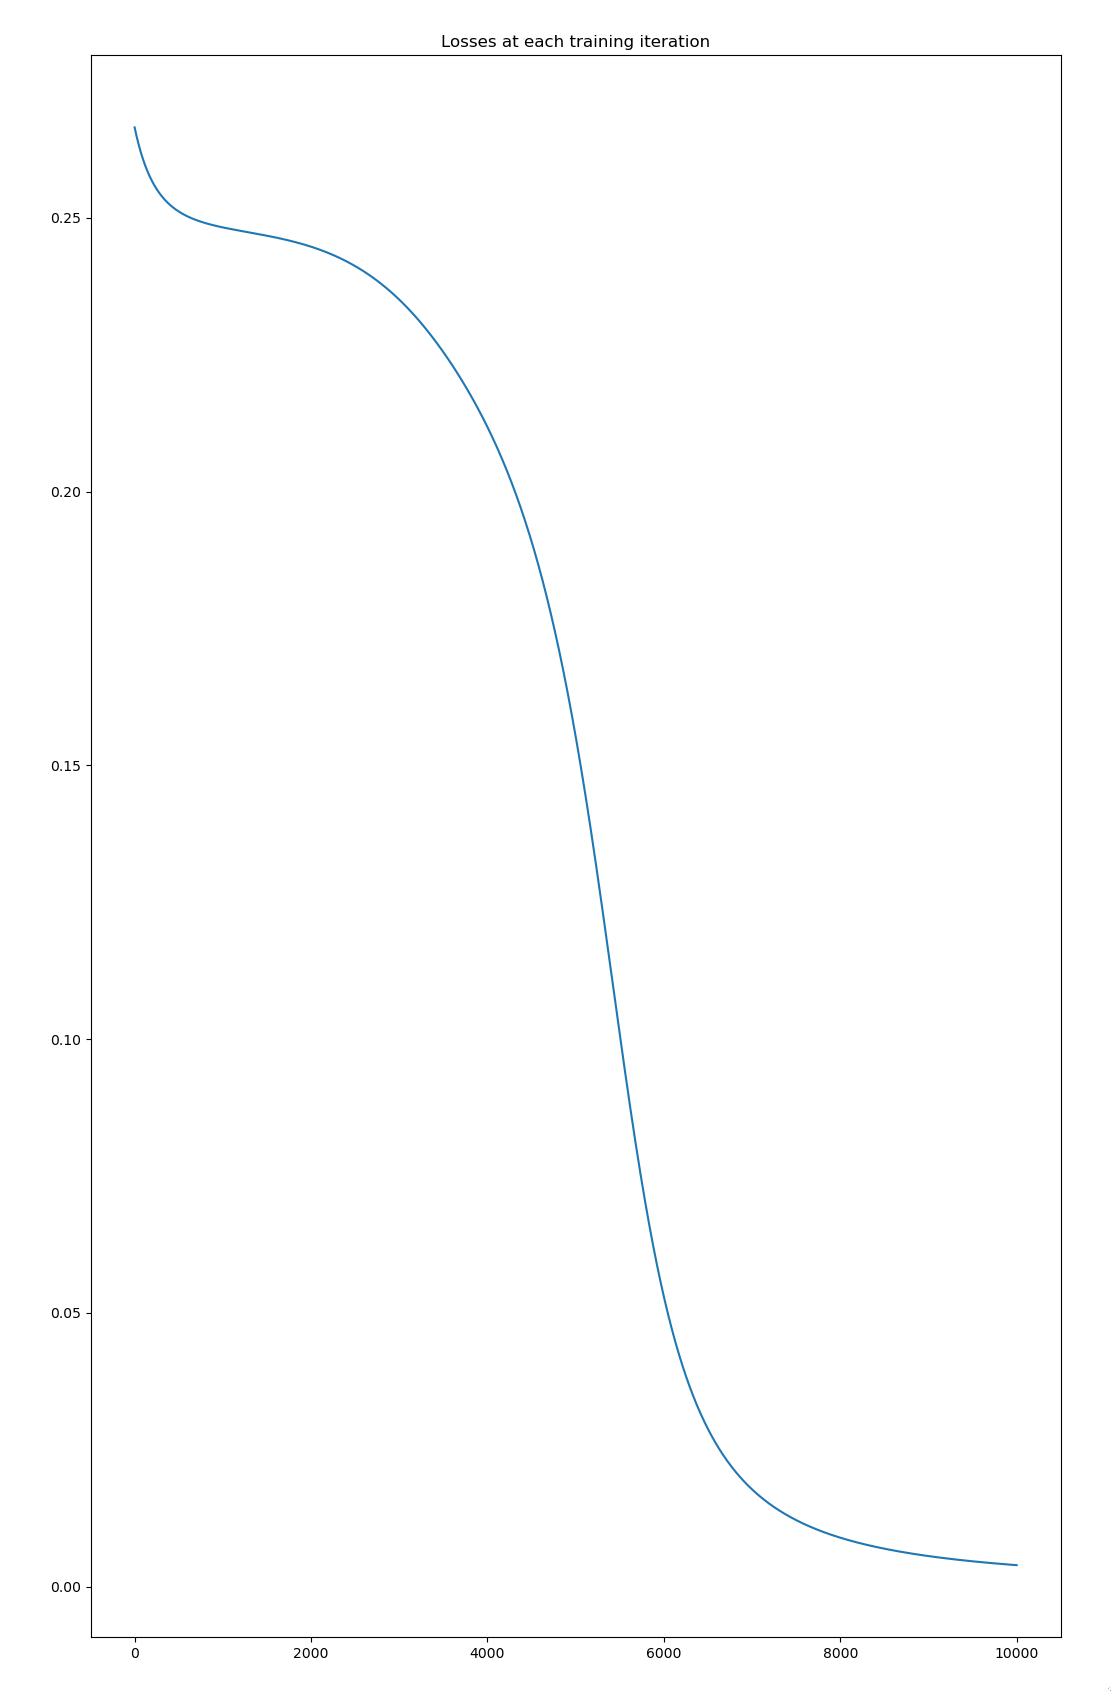
\includegraphics[width=0.3\textwidth]{./media/loss_function_initial_nn.png}
\caption{\label{fig:org5f8c32b}Training error, given by \(l\left( x \right) = \sum^{n}_{i= 1} \left[ \left( x_i - f\left( x_i \right)  \right)^2  \right]\), at each iteration of training}
\end{figure}

\subsection{Implement Ranknet\hfill{}\textsc{f25f376:05df04f}}
\label{sec:org443cd25}
Now that the model can classify the data, the implementation will
be modified to:

\begin{itemize}
\item Measure loss using a BCE function which is reported to perform better in the
literature \cite{christopherburgesRankNetRankingRetrospective2015,christopherburgesRankNetLambdaRankLambdaMART2010}
\item Modify the model so that it operates pairwise, such that:
\begin{enumerate}
\item Two points are identified, sent through the neural network and
two values returned:
\begin{align}
s_i = n(\mathbf{X}_i) \label{eq:forward_single1}\\
s_j = n(\mathbf{X}_j) \label{eq:forward_single2}
\end{align}
The network previously created can be adapted for this and
hence the method will be renamed to \texttt{forward\_single} and this
will represent function \(n()\) implemented in
\eqref{eq:forward_single1} and \eqref{eq:forward_single2}
\item These values will be combined to give a single value which is
intended to measure the model confidence:\footnote{This value is a measurement of the models "confidence" but
could be extended to represent the "measured probability" of one item
being ranked higher than an other (e.g. the probability that a person
would rank one type of wine as better than the other in a random
sample).}

\begin{align}
\hat{P}_{ij} &= \mathrm{sig}\left(\sigma, (s_i-s_j)\right), \quad
\exists \sigma \in \mathbb{R} \\
&= \frac{1}{1+e^{\sigma \cdot (s_i-s_j)}} \label{eq:sig-comb}
\end{align}
\item The range of \eqref{eq:sig-comb}  is the interval \(\hat{P}_{ij} =
        \left[0, 1\right]\), let \(\bar{P}_{ij}\) be the known
probability\footnote{Note the convention that the symbols \(\triangleleft, \enspace \triangleright\) have been adopted to denote the ranking of two observations,
analogous to \(<, \enspace >\)} that \(\mathbf{X}_i \triangleright
        \mathbf{X}_j\), the simulated data has a boolean range of
\(\bar{P}_{ij} \in \left\{0, 1\right\}\), this can be recast
to \(\{-1, 0, 1\}\) and then linearly scaled to \(\left[0,
        1\right]\) like so:

\begin{align}
\bar{P}_{ij} & \leftarrow p_i - p_j \\
\bar{P}_{ij} & \leftarrow \frac{1+\bar{P}_{ij}}{2}
\end{align}
\end{enumerate}
\end{itemize}


These modifications only need to be made to the neural network
class like so:

\begin{minted}[]{python}
class three_layer_ranknet_network(nn.Module):
    # __init__ method
    # ...
    # ...

    def forward(self, xi, xj):
	si = self.forward_single(xi)
	sj = self.forward_single(xj)
	out = 1 / (1 + torch.exp(-self.σ * (si - sj)))  
	return out

    def forward_single(self, x):
	x = torch.matmul(x, self.wi).add(self.bi)
	x = torch.sigmoid(x)
	x = torch.matmul(x, self.wo).add(self.bo)
	x = torch.sigmoid(x)

	return x

    def loss_fn(self, xi, xj, y):
	y_pred = self.forward(xi, xj)
	loss = torch.mean(-y * torch.log(y_pred) -
			  (1 - y) * torch.log(1 - y_pred))
	return loss

   def pairwise(iterable):
       "pairwise([1,2,3,4]) --> [(1, 2), (1, 3), (1, 4), (2, 3), (2, 4), (3, 4)]"
       s = list(iterable)
       pair_iter = chain.from_iterable(combinations(s, r) for r in [2])
       return pair_iter

\end{minted}

The training method must be adapted to interact with these changes
like so:\footnote{Note the definition of the \texttt{pairwise} function, this was
incorrectly implemented initially (\texttt{f25f376}) and rectified shortly
after (\texttt{05df04f}). see \ref{sec:org4d8baca}}

\begin{minted}[]{python}
class three_layer_ranknet_network(nn.Module):
    # __init__ method
    # ...
    # ...
    def train(self, x, target, η=1e-2, iterations=4e2):
	self.trainedQ = True
	# Create a progress bar
	bar = Bar('Processing', max=iterations)
	# Train for a number of iterations
	for t in range(int(iterations)):
	    sublosses = []
	    # Loop over every pair of values
	    for pair in pairwise(range(len(x) - 1)):
		xi, yi = x[pair[0], ], target[pair[0]]
		xj, yj = x[pair[1], ], target[pair[1]]

		# encode from {0, 1} to {-1, 0, 1}
		y = yi - yj

		# Scale between {0,1}
		y = 1 / 2 * (1 + y)

		# Calculate y, forward pass
		y_pred = self.forward(xi, xj)

		# Measure the loss
		loss = self.loss_fn(xi, xj, y)
		sublosses.append(loss.item())

		# Calculate the Gradients with Autograd
		loss.backward()

		# Update the Weights with Gradient Descent
		# ; Zero out the gradients, they've been used
		with torch.no_grad():
		    self.wi -= η * self.wi.grad; self.wi.grad = None
		    self.bi -= η * self.bi.grad; self.bi.grad = None
		    self.wo -= η * self.wo.grad; self.wo.grad = None
		    self.bo -= η * self.bo.grad; self.bo.grad = None
		    self.σ  -= η * self.σ.grad ; self.σ.grad  = None

	    self.losses.append(np.average(sublosses))
	    bar.next()
	bar.finish()
	self.threshold_train(x, target, plot=False)
\end{minted}

This can then be implemented as before with the loss function shown
in figure , one of the greatest difficulties in
implementing this, however, is that it is not simple to determine
whether or not the model has classified the data well:\footnote{A naive misclassification method was implemented (\texttt{f25f376}),
but it was not very insightful and so was omitted from this report.} 

\begin{minted}[]{python}
# Make the Data
X_train, X_test, y_train, y_test = make_data(
    n=30, create_plot=True, dtype=dtype, dev=dev)

# Create a model object
model = three_layer_ranknet_network(
    input_size=X_train.shape[1], hidden_size=2, output_size=1, dtype=dtype, dev=dev)

# Train the Model
model.train(X_train, y_train, η=1e-1, iterations=1e2)

# Save the losses
np.savetxt(fname="/tmp/losses.csv", X=model.losses, delimiter=',')

\end{minted}

\subsection{Implement sorting}
\label{sec:org34e0868}
So instead of ranking, sort the values, this produces the output.

but this is the problem, did it work? it's not clear, because even
if the model was not trained we get the following (put them side by side).

So this is definitely one of the hard issues.

what would be better would be to classify data with a rating
(i.e. wine scores), only show the model whether the wine is
good/bad and compare the output order with the input order, that
would be an effective way to see that it works. This was not yet
effectively implemented.
\subsection{Moons}
\label{sec:org64db56f}
\subsection{Optimisers}
\label{sec:org0362e30}
\subsection{Batches}
\label{sec:org21a7e61}
\subsection{Wine}
\label{sec:org7a10a93}
\subsection{Rank Wiki Articles}
\label{sec:org5a6ad60}
\section{Difficulties}
\label{sec:orgda7e9db}
\begin{itemize}
\item Don't use torch
\begin{itemize}
\item Do it by hand first because it can be hard to see if the correct
weights are being updated sensibly, making debugging very difficult.
\item R or Julia would be easier because counting from 0 get's pretty
confusing when dealing with \{1, 0\}, \{-1, 0, 1\}.
\end{itemize}
\item Don't use misclassification rate to measure whether the ranking
\begin{itemize}
\item In hindsight this is obvious, but at the time misclassification
was a tempting metric because of it's interpretability
\end{itemize}
was correct

Very difficult to see if the model is working

\item A continuous function will still produce an ordered pattern in
the ranking of results, even if the model hasn't been trained,
so visualising isn't helpful either.

\item Implement it on a data set that already has order, obfuscate the
order and then contrast the results
\begin{itemize}
\item or use a measurement
\end{itemize}

\item Plot the loss function of the training data live, the model is
slow to train and waiting for it to develop was a massive time
drain.
\end{itemize}



\section{Further Research}
\label{sec:org34c687f}


\subsection{Practical Improvements}
\label{sec:orgb11772e}

\begin{itemize}
\item Apply this to documents to get a sorted list, like the wine data
\item The "Quicksort" algorithm likely needs a random pivot to be efficient \cite{timroughgardenQuicksortOverview2017}
\end{itemize}

\subsection{Evaluate performance improvements}
\label{sec:orgab5dd90}

It is still not clear how the
performance of Ranknet compares to traditional approaches
implemented by search engines (see \S \ref{sec:orgc3c7fd7}), further
study would ideally:

\begin{itemize}
\item Write a program to query a corpus of documents using an existing search engine.
\begin{itemize}
\item Or possibly just implement TF-IDF weighting in order to remove variables.
\end{itemize}
\item Extend the program to implement machine learned ranking
\item Measure and contrast the performance of the two models to see
whether there are any significant improvements.
\end{itemize}

This could be implemented with TREC datasets
\cite{usnationalinstituteofstandardsandtechnologyTextREtrievalConference}
using a cummulated-gain cost function
\cite{jarvelinCumulatedGainbasedEvaluation2002} as demonstrated in
previous work \cite{viksinghComparisonOpenSource2009}.

\subsection{Evaluate alternative machine learning models}
\label{sec:orgbab0c14}
i.e. can SVM's or trees be used instead of neural networks?

\section{Conclusion}
\label{sec:org903930c}

\section{Text and References}
\label{sec:orgd352a7f}
Fractals are complex shapes that often occur from natural processes, in this
report we hope to investigate the emergence of patterns and complex structures
from natural phenomena. We begin with an investigation into fractals and the
concept of dimension and then discuss links between fractal patterns and natural
processes.

This is a Reference \cite{tuGraphBasedSemiSupervisedNearestNeighbor2016a} and another \cite{nicodemiIntroductionAbstractAlgebra2007a} and yet another \cite{christopherburgesRankNetLambdaRankLambdaMART2010}.

\section{Fractals}
\label{sec:org1c22a6e}
Images are shown in figure .

\section{Appendix}
\label{sec:org6aeab4e}

\subsection{Search Engines}
\label{sec:orgc3c7fd7}
There are many open source search engines available , a cursory review
found the following popular projects:

\begin{itemize}
\item \href{https://github.com/cyclaero/zettair}{Zettair} (\texttt{C}) \cite{jansenCyclaeroZettair2020}
\item \href{https://github.com/apache/lucene-solr}{Apache lucene/Solr} (\texttt{Java}) \cite{apachesoftwarefoundationLearningRankApache2017}
\begin{itemize}
\item Implemented by \href{https://sourceforge.net/p/docfetcher/code/ci/master/tree/}{DocFetcher} \cite{docfetcherdevelopmentteamDocFetcherFastDocument}
\end{itemize}
\item \href{https://github.com/sphinxsearch/sphinx}{Sphinx} (\texttt{C++}) \cite{yurischapovSphinxsearchSphinx2021}
\item \href{https://github.com/kevinduraj/xapian-search}{Xapian} (\texttt{C++}) \cite{ollybettsXapianXapian2021}
\begin{itemize}
\item Implemented by \href{https://www.lesbonscomptes.com/recoll/}{Recoll} \cite{jean-francoisdockesRecollUserManual}
\end{itemize}
\end{itemize}

More Modern Search engines include:

\begin{itemize}
\item \href{https://github.com/olivernn/lunr.js/}{LunrJS}  (\texttt{JS}) \cite{nightingaleOlivernnLunrJs2021}
\item \href{https://github.com/blevesearch/bleve}{Bleve Search} (\texttt{Go}) \cite{martyschochBleveSearchDocumentation}
\item \href{https://github.com/go-ego/riot}{Riot} (\texttt{Go}) \cite{vzGoegoRiot2021}
\item \href{https://github.com/tantivy-search/tantivy}{Tantivy} (\texttt{Rust}) \cite{clementrenaultMeilisearchMeiliSearch2021}
\item \href{https://github.com/andylokandy/simsearch-rs}{SimSearch} (\texttt{Rust}) \cite{lokAndylokandySimsearchrs2021}
\end{itemize}


\subsubsection{Fuzzy String Match}
\label{sec:org643c970}
Somewhat related are programs that rank string similarity, such programs don't tend
to perform well on documents however (so for example these would
be effective to filter document titles but would not be useful for
querying documents):

\begin{itemize}
\item \href{https://github.com/junegunn/fzf}{\texttt{fzf}} \cite{choiJunegunnFzf2021}
\item \href{https://github.com/jhawthorn/fzy}{\texttt{fzy}} \cite{hawthornJhawthornFzy2021}
\item \href{https://github.com/peco/peco}{\texttt{peco}} \cite{lestrratPecoPeco2021}
\item \href{https://github.com/lotabout/skim}{Skim} \cite{zhangLotaboutSkim2021}
\item \href{https://github.com/lotabout/skim}{\texttt{go-fuzzyfinder}} \cite{ktrKtr0731Gofuzzyfinder2021}
\item \href{https://github.com/lotabout/skim}{Swiper} \cite{krehelAboaboSwiper2021}
\end{itemize}

\subsection{Import Statements}
\label{sec:orgd262b36}
The following import statements were included, where used, \footnote{Including \texttt{import} statements where they are not used is fine,
other than complaints from a \emph{linter} following \emph{PEP}
\cite{nickcoghlanPEPStyleGuide2001} (e.g. \href{https://pypi.org/project/autopep8/}{autopep}
\cite{hattoriAutopep8ToolThat}) the code will function just fine.}
separate scripts were used to make the model as modular as possible,
such corresponding inputs have also been listed:

\begin{minted}[]{python}
# Import Packages
from itertools import chain
from itertools import combinations
from itertools import tee
from progress.bar import Bar
import math as m
import matplotlib.pyplot as plt
import numpy as np
import random
import sys
import sys
import torch
import torch
from torch import nn

# Sepereate Scripts lcated below main
from ranknet.test_cuda import test_cuda
from ranknet.make_data import make_data
from ranknet.neural_network import three_layer_ranknet_network
from ranknet.quicksort import quicksort
\end{minted}

\subsection{Export Data Method}
\label{sec:org66415ad}
The data was exported by printing the values to a text file like
so:

\begin{minted}[]{python}
def export_data(X, y, export):
    try:
	os.remove(export)
	print("Warning, given file was over-written")
    except:
	pass

    with open(export, "a") as f:
	line = "x1, x2, y \n"
	f.write(line)
	for i in (range(X.shape[0])):
	    line = str(X[i][0]) + ", " + str(X[i][1]) + ", " + str(y[i]) + "\n"
	    f.write(line)
    print("Data Exported")


\end{minted}

\subsection{Version Control Repository}
\label{sec:org466ef15}
The \texttt{git} repository used in production of this code is currently
available on \emph{GitHub} at \href{https://github.com/CRMDS/CRMDS-HDR-Training-2020}{github.com/CRMDS/CRMDS-HDR-Training-2020}, in
order to get a local copy, execute the following commands (\texttt{bash}): 

\begin{minted}[]{bash}
# Clone the repository
git clone https://github.com/CRMDS/CRMDS-HDR-Training-2020

# Change to the subdirectory
cd CRMDS-HDR-Training-2020/ranknet

# Checkout the Walkthrough branch
git checkout walkkthrough

# list the changes
git log
\end{minted}

Consider the use of tools like \href{https://magit.vc/}{magit} \cite{MagitMagit2008} and
\href{https://github.com/emacsmirror/git-timemachine}{git-timemachine} \cite{peterstiernstromEmacsmirrorGittimemachine2014} (or
\href{https://marketplace.visualstudio.com/items?itemName=eamodio.gitlens}{GitLens} \cite{amodioEamodioVscodegitlens2016} and \href{https://marketplace.visualstudio.com/items?itemName=bee.git-temporal-vscode}{git-temporal}
\cite{beewilkersonGittemporalGittemporalMono2018} in VsCode) in order
to effectively preview the changes at each step, alternatively a
pager like \href{https://github.com/sharkdp/bat}{bat} \cite{peterSharkdpBat2018} can also be used with something like \href{https://github.com/junegunn/fzf}{fzf}
\cite{choiJunegunnFzf2021} like so:

\begin{minted}[]{bash}
git log | grep '^commit' | sed 's/^commit\ //' |\
    fzf --preview 'git diff {}^! |\
     bat --color always'  
\end{minted}

\subsubsection{Version Control Log for Walkthrough}
\label{sec:org4d8baca}
\begin{center}
\begin{tabular}{ll}
\textbf{\emph{Commit ID}} & \textbf{\emph{Message}}\\
\hline
\texttt{ed5f4cf} & \emph{Initial Commit}\\
\texttt{075acf9} & \emph{Walkthrough Initial Commit}\\
\texttt{cf9ab26} & \emph{Generate data to use for classification}\\
\texttt{7291112} & \emph{Create a Neural Network Model}\\
\texttt{7d46636} & \emph{Implement gradient descent to train neural network}\\
\texttt{f25f376} & \emph{Adapt Neural Network to perform Ranking}\\
\texttt{42509ab} & \emph{Implement sorting algorithm to visualise ranking order}\\
\texttt{05df04f} & \emph{Adapt Neural Network to perform Ranking}\\
\texttt{99b390a} & \emph{Implement sorting algorithm to visualise ranking order}\\
\texttt{473dce3} & \emph{Implement optimizer to replace mere gradient descent}\\
\texttt{4141e92} & \emph{Train Model using Batches not entire dataset}\\
\texttt{a2671a6} & \emph{Format code to make it more readable}\\
\texttt{d11e607} & \emph{plot and only train on different ranked pairs}\\
\end{tabular}

\end{center}
\end{document}